%!TEX root = ../hutbthesis_main.tex
\chapter{机场牵引车辆系统建模与问题理论基础}

\section{机场牵引作业场景抽象}

机场牵引作业通常发生在停机位、廊桥附近和机坪连接滑行通道区域。与普通道路车辆行驶相比，牵引车的运行速度很低，但控制难度并不低：车辆要在有限空间内靠近飞机前起落架，既要避免车体、机翼和地面保障设备之间发生干涉，又要保证车头方向、横向位置和停车距离满足后续机械连接要求。对于本课题中的双桥转向牵引车而言，前后转向桥能够提高机动性，但也使车辆运动模式和控制输入之间的关系更加复杂。

结合本文研究目标，可将自动牵引对接过程抽象为五个连续阶段。第一阶段为任务初始化与目标确认，牵引车接收目标飞机信息并通过辅助识别标识完成身份判断；第二阶段为初始接近，车辆从给定初始位姿向飞机前起落架附近的预对接区域运动；第三阶段为姿态对准，车辆重点减小横向偏差和航向误差，使车体中心线逐步贴近目标对接方向；第四阶段为微动对接，牵引车在低速状态下完成小范围位置修正；第五阶段为停车保持，系统在满足距离、姿态和安全阈值后发布停车与转向回中命令。

由此可见，飞机推出不是一条轨迹从起点跟到终点这么简单，而是目标识别、车辆运动学约束、安全边界和模式切换共同作用的状态演化过程\textsuperscript{[17-21]}。本章只先处理牵引车本体在机坪平面内如何运动的问题，即建立位姿状态、曲率关系和输入约束；飞机辅助识别、局部安全判断和最终对接控制将在第三章统一展开。

\section{坐标系与状态变量定义}

为统一描述牵引车在机坪平面内的运动状态，建立全局惯性坐标系
\(O\text{\,} - \text{\,}XY\)与车体坐标系
\(C\text{\,} - \text{\,}xy\)。其中，全局坐标系固定于地面，主要用于描述车辆在场景中的绝对位置；车体坐标系原点取在车辆参考点
\(C\)处，该点可取车辆几何中心、质心或控制参考中心，\(x\)
轴沿车辆纵向前进方向，\(y\) 轴沿车辆横向方向。

定义车辆位姿状态为\(\mathbf{q} = \begin{bmatrix}
x & y & \theta
\end{bmatrix}^{T}\) 。其中，\(x\) 与
\(y\)分别表示车辆参考点在全局坐标系中的位置坐标，\(\theta\)
表示车体纵向轴相对于全局
\(X\)轴的夹角，即车辆航向角。进一步地，为描述车辆运动过程中的速度状态，引入线速度
\(v\)作为系统运动输入或状态扩展量，则可将系统状态写为\(\mathbf{x} = \begin{bmatrix}
x & y & \theta & v
\end{bmatrix}^{T}\) 。式中\(v\)
表示车辆沿车体纵向的速度分量。该状态定义方式具有两点作用：一方面，\(\left( x,y,\theta \right)\)
可直接用于描述车辆轨迹；另一方面，\(v\)
可与转向输入共同决定系统状态的实时演化。

对于本课题所研究的双桥转向牵引车，前桥和后桥均具有独立转向能力，因此进一步定义前桥转角与后桥转角分别为
\(\delta_{f}\)与
\(\delta_{r}\)。若将系统控制输入写为\(\mathbf{u} = \begin{bmatrix}
v & \delta_{f} & \delta_{r}
\end{bmatrix}^{T}\)，则后续运动学模型即可统一写成关于 \(\mathbf{x}\)与
\(\mathbf{u}\)的非线性状态方程。

\section{车辆运动学模型建立}

\subsection{非完整约束条件}

牵引车在机坪低速运行过程中，车轮主要满足纯滚动约束，即轮胎可沿轮平面方向滚动，但不能在垂直于轮平面的方向上发生理想横向滑移。因此，车辆系统属于典型非完整约束系统。对于车体参考点
\(C\)，其速度在车体横向方向上的投影应为零，可写为\(\dot{y}\cos\theta - \dot{x}\sin\theta = 0\)。该式的物理意义在于：车辆不能瞬时``侧向平移''，其平面运动只能由纵向速度与航向变化共同形成。这一约束是移动机器人与地面车辆运动学建模中的基本条件，也是后续推导轨迹方程的前提\textsuperscript{[17,19]}。

\subsection{单轨等效模型}

由于前桥左右轮、后桥左右轮在同一转向控制下可近似视为对称运动，因此可采用单轨等效方法，将实际四轮结构抽象为前后两虚拟轮\textsuperscript{[19]}。设前、后桥中心点分别位于车体参考点前后，车辆轴距为
\(L\)。在低速、小侧偏工况下，车辆瞬时旋转中心满足几何关系，车辆平面运动可表示为（1）

\(\left\{ \begin{array}{r}
\dot{x} = vcos\theta \\
\dot{y} = vsin\theta \\
\dot{\theta} = \omega\ 
\end{array} \right.\ \) （1）

式中，\(\omega\)
为车辆偏航角速度。前两式给出了车辆质点速度在全局坐标系中的分解形式，第三式给出了车辆姿态随时间的演化规律。车辆轨迹由两个因素共同决定：一是沿当前朝向的平移速度
\(v\)，二是决定航向变化速率的角速度 \(\omega\)。

\subsection{双桥转向角速度表达式}

对于普通前轮转向车辆，角速度通常由单一前轮转角决定；而对于双桥转向车辆，前桥和后桥转向均会对瞬时旋转中心位置产生影响。根据单轨几何关系，前桥与后桥分别对应的曲率贡献为
\(\tan\delta_{f}/L\)与
\(\tan\delta_{r}/L\)。在统一参考方向下，车辆偏航角速度可表示为：\(\dot{\theta} = \omega = \frac{v}{L}\left( \tan\delta_{f} - \tan\delta_{r} \right)\)。\(\delta_{f}\)
为前桥转角，\(\delta_{r}\) 为后桥转角，\(L\)
为前后桥中心距。该式表明，前桥转向与后桥转向对车辆角速度的作用方向相反。当后桥不转向，即
\(\delta_{r} = 0\)时，模型退化为普通前轮转向模型；当前后桥反向转向时，\(\tan\delta_{f} - \tan\delta_{r}\)
的绝对值增大，车辆角速度提高，转弯半径减小；当前后桥同向转向时，两者效应相互抵消，车辆偏航角速度下降，车辆运动趋于``蟹行''模式。

将上述关系代入状态方程，可得双桥转向牵引车的运动学模型（2）

\(\left\{ \begin{array}{r}
\dot{x} = vcos\theta \\
\dot{y} = vsin\theta \\
\dot{\theta} = \frac{v}{L}\left( tan\delta_{f} - tan\delta_{r} \right)
\end{array} \right.\ \) （2）

该模型是本课题后续路径规划、轨迹跟踪与对接控制设计的基础模型\textsuperscript{[17,19,28]}。

\section{转弯半径与曲率模型}

车辆轨迹几何特性通常由曲率或转弯半径刻画。设车辆瞬时转弯半径为
\(R\)，则有

\begin{equation}
\omega = \frac{v}{R}
\tag{3}
\label{eq:3}
\end{equation}

结合上一节所得角速度表达式，可得双桥转向牵引车的等效转弯半径为

\begin{equation}
R = \frac{L}{\tan\delta_{f} - \tan\delta_{r}}
\tag{4}
\label{eq:4}
\end{equation}

若进一步定义轨迹曲率 \(\kappa\)为转弯半径的倒数，则有

\begin{equation}
\kappa = \frac{1}{R} = \frac{\tan\delta_{f} - \tan\delta_{r}}{L}
\tag{5}
\label{eq:5}
\end{equation}

上述两式给出了车辆转向输入与轨迹几何属性之间的直接联系。式中，\(R\)
用于衡量车辆完成转弯所需空间尺度，\(R\)
越小，表明车辆机动性越强；\(\kappa\) 用于衡量轨迹弯曲程度，\(\kappa\)
越大，表明车辆航向变化越快。对机场牵引作业而言，车辆能否在狭窄区域内完成姿态调整，本质上取决于其可实现的最小转弯半径或最大曲率\textsuperscript{[19,28]}。

需要指出的是，理论上当
\(\tan\delta_{f} - \tan\delta_{r} = 0\)时，\(R \rightarrow \infty\)，车辆轨迹退化为直线或近似平移；而当
\(\mid tan\delta_{f} - \tan\delta_{r} \mid\)增大时，车辆可实现更强的转向能力。但在工程应用中，前后桥转角均受机械结构、执行器能力和稳定性要求限制，因此曲率不可能无限增大，而必须满足可实现性约束。

\section{典型转向模式分析}

双桥转向车辆较普通单桥转向车辆具有更丰富的运动模式。为明确不同转向策略对车辆机动性的影响，分别讨论以下三种典型工况。

\subsection{前桥单独转向模式}

当后桥不参与转向，即\(\delta_{r} = 0\)时，车辆运动学模型退化为

\begin{equation}
\dot{\theta} = \frac{v}{L}\tan\delta_{f}
\tag{6}
\label{eq:6}
\end{equation}

此时车辆行为与传统前轮转向车辆基本一致（图2-1）。该模式实现简单、控制逻辑清晰，但在对接空间受限的场景下，其最小转弯半径较大，不利于快速完成姿态调整。

\begin{figure}[htbp]
    \centering
    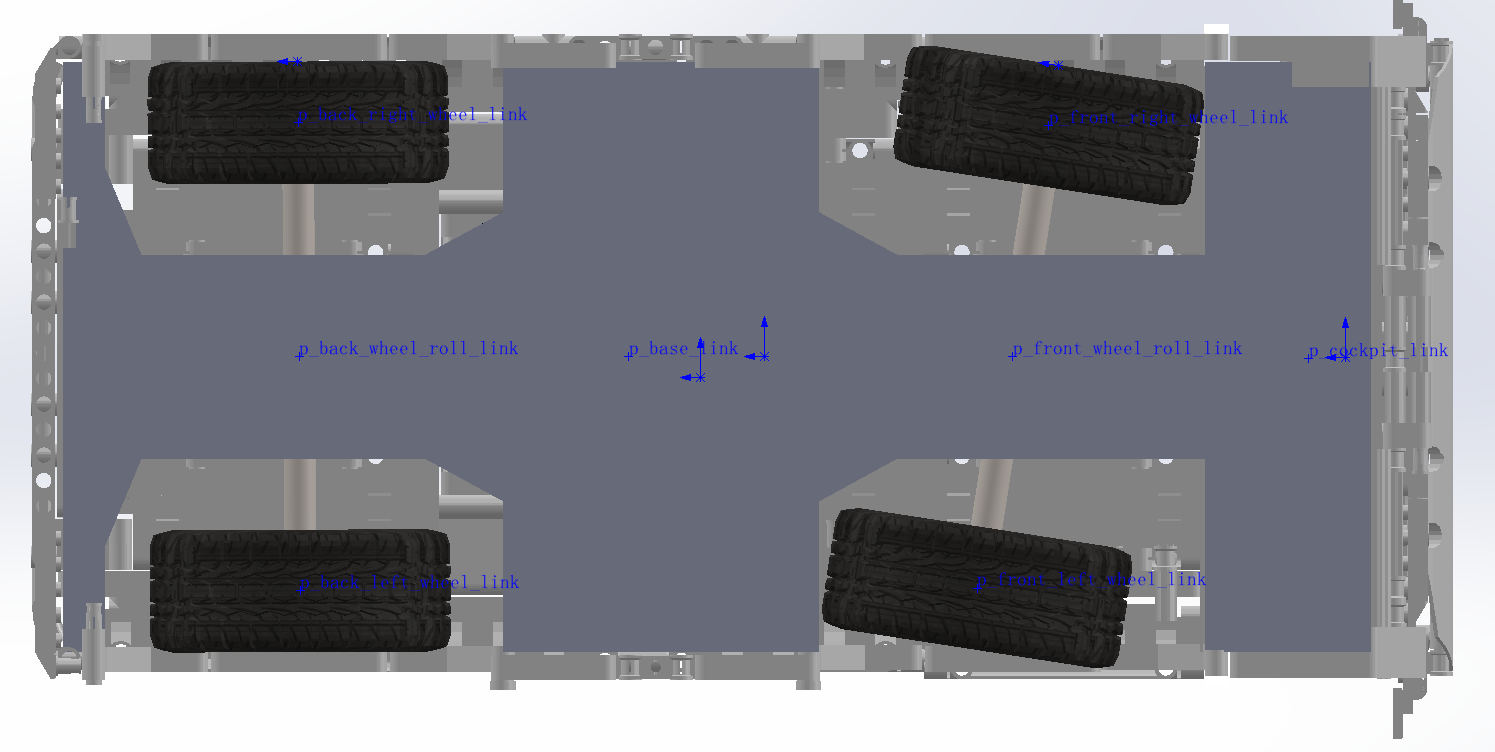
\includegraphics[width=4.66955in,height=2.12251in]{figures/image3.png}
    \caption{传统转向模式}
    \label{fig:2-1}
\end{figure}

\subsection{前后桥反向转向模式}

当后桥转角与前桥转角方向相反，且幅值近似相等，即\(\delta_{r} = - \delta_{f}\)代入角速表达式可得

\(\dot{\theta} = \frac{v}{L}\left( tan\delta_{f} - tan( - \delta_{f}) \right) = \frac{2v}{L}tan\delta_{f}\)
（7）

此时车辆偏航角速度约为单桥转向工况的两倍，转弯半径显著减小（图2-2），适用于牵引车在狭小机坪空间内快速调整姿态、靠近飞机前轮或完成局部避障。该模式是本课题中实现高机动性接近控制的重要运动模式。

\begin{figure}[htbp]
    \centering
    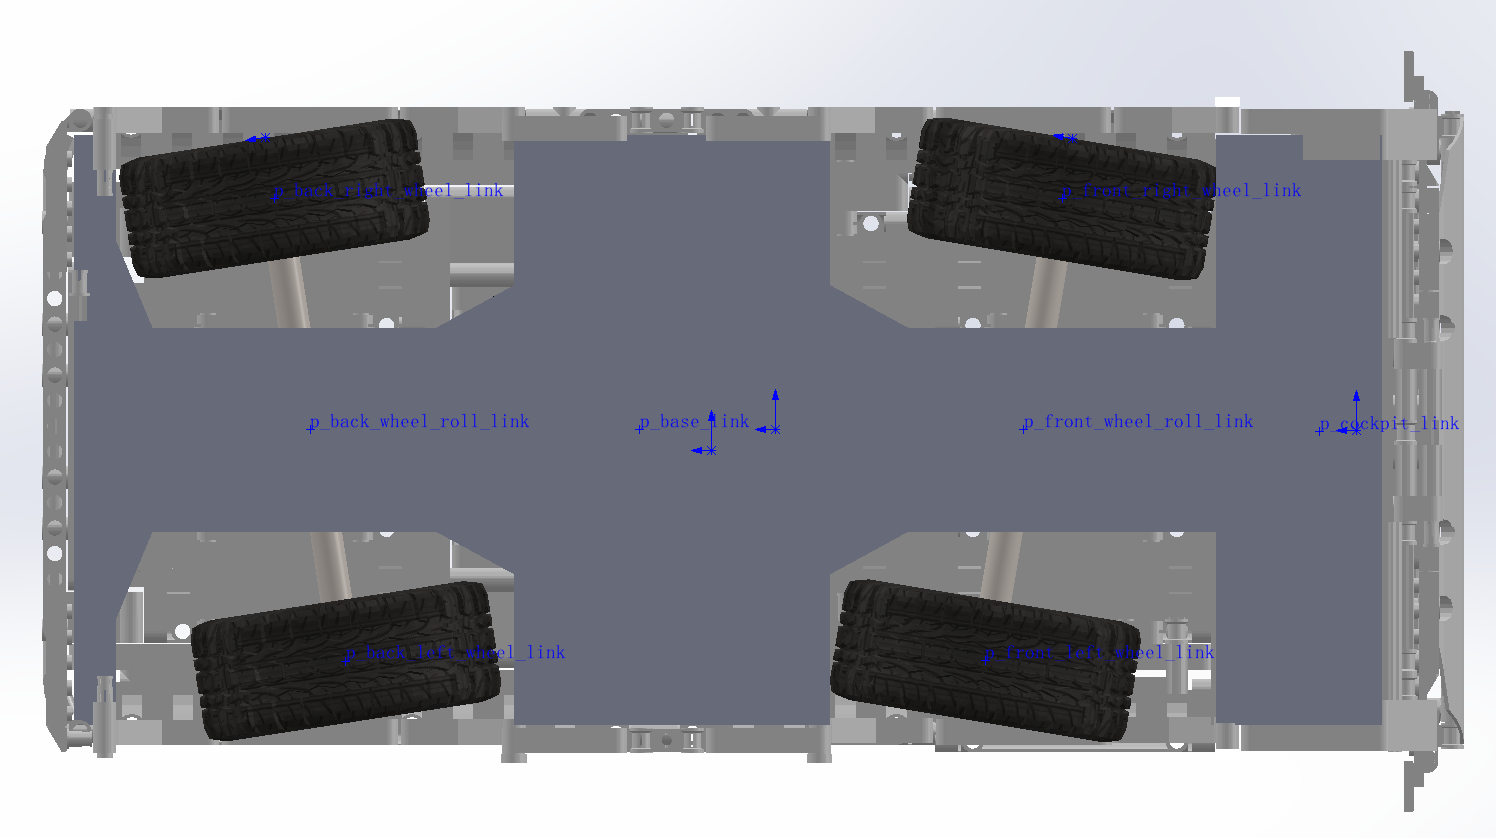
\includegraphics[width=5.05627in,height=2.29662in]{figures/image4.png}
    \caption{前后桥反向转向模式}
    \label{fig:2-2}
\end{figure}

\subsection{前后桥同向转向模式}

当\(\delta_{r} = \delta_{f}\)时，有\(\dot{\theta} = \frac{v}{L}\left( \tan\delta_{f} - \tan\delta_{f} \right) = 0\)

当车辆偏航角速度为零，此时车辆整体保持原有航向并沿车轮切线方向斜向平移，表现为
``蟹行''运动（图2-3）。该模式并不适合大幅姿态修正，但对于微小横向误差修正、精细对位和低速贴近控制具有较高实用价值。

通过上述分析可知，双桥转向结构使牵引车不再局限于单一的``直行---转弯''运动，而具备在姿态快速修正与横向精细调节之间切换的能力，这也是其适用于飞机自动对接场景的重要原因。

\begin{figure}[htbp]
    \centering
    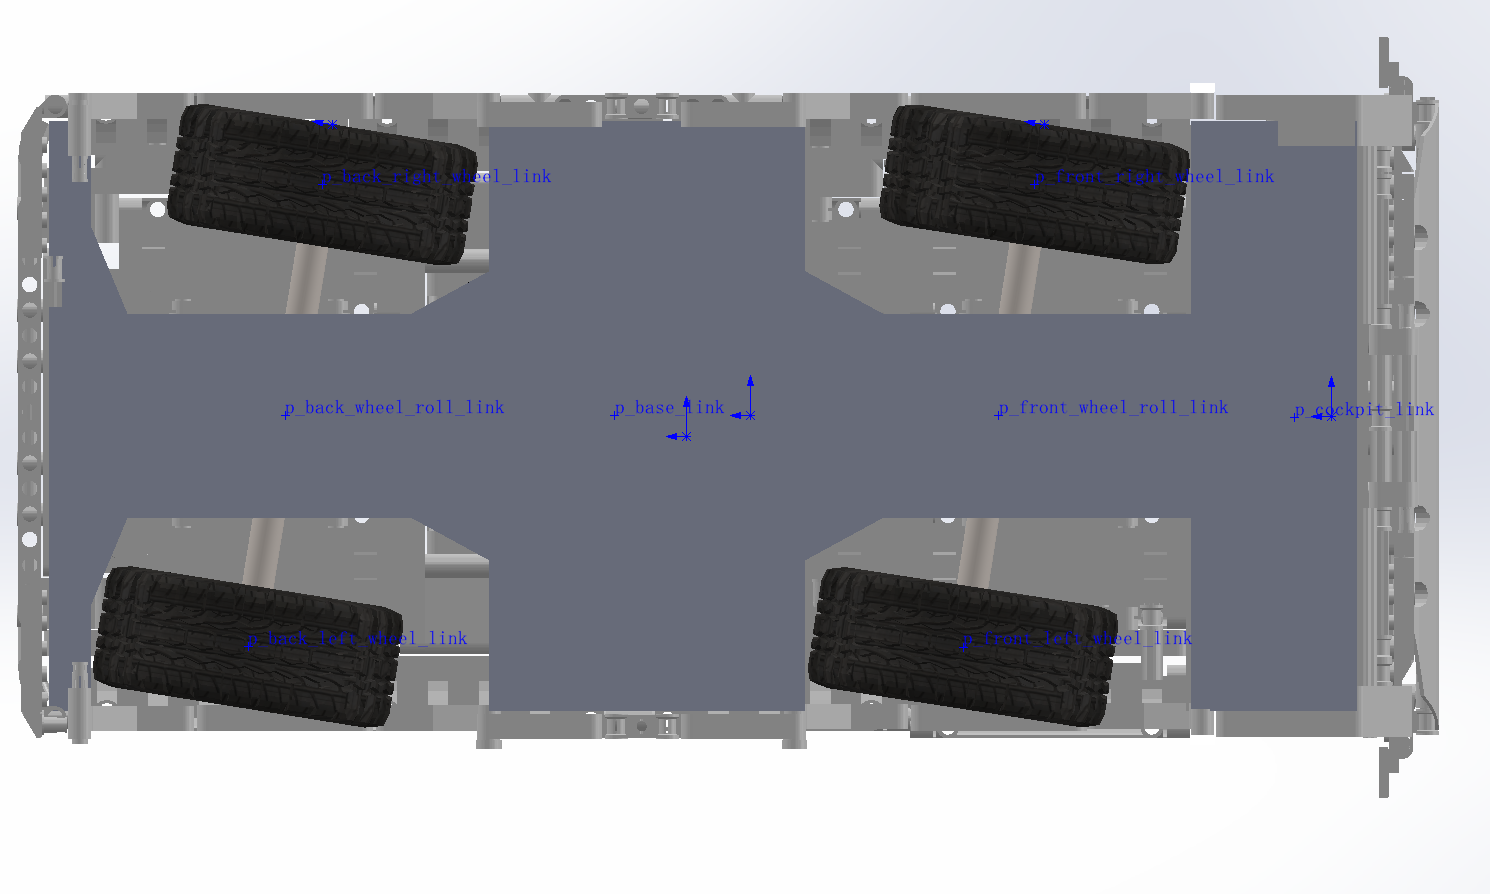
\includegraphics[width=4.99734in,height=2.27042in]{figures/image5.png}
    \caption{前后桥同向转向模式}
    \label{fig:2-3}
\end{figure}

\section{速度、转角与曲率约束建模}

运动学模型给出了系统状态演化规律，但在实际推引作业中，车辆运动必须满足结构约束与运行约束。因此，需要进一步建立输入与状态约束。

\subsection{速度约束}

牵引车在机场作业环境中通常处于低速运行状态，故其线速度应满足\(0 \leq v \leq v_{\max}\)
。

其中，\(v_{\max}\)
为车辆允许的最大作业速度。该约束保证车辆在接近、对接和牵引过程中具有足够的可控性，同时减小碰撞风险。

\subsection{转向角约束}

由于前后桥转向机构存在机械极限，故应满足

\(\left\{ \begin{array}{r}
 \mid \delta_{f} \mid \leq \delta_{f,max} \\
 \mid \delta_{r} \mid \leq \delta_{r,max}
\end{array} \right.\ \) （8）

其中，\(\delta_{f,\max}\) 与
\(\delta_{r,\max}\)分别为前桥与后桥最大允许转角。该约束直接限制车辆最大可实现曲率，也是最小转弯半径存在下界的原因。

\subsection{曲率约束}

由转向角约束可进一步得到曲率约束\(\mid \kappa \mid \leq \kappa_{\max}\)。其中，

\(\kappa_{\max} = \frac{tan\delta_{f,max} - tan( - \delta_{r,max})}{L}\)
（9）

当车辆采用对称反向转向策略时，上式取到较大值。曲率约束在路径规划中具有重要作用，因为若规划轨迹的局部曲率超过车辆可实现上限，则该轨迹在物理上不可执行\textsuperscript{[20-21,28]}。

\section{车辆动力学简化与驱动关系}

本课题以低速自主牵引控制为研究重点，后续控制层主要关注位姿演化与轨迹误差收敛，因此在第二章中不引入完整轮胎力学模型，而仅保留纵向驱动的简化动力学关系\textsuperscript{[19]}。设车辆等效质量为
\(m\)，驱动力为 \(F\)，纵向加速度为 \(a\)，则有\(F = ma\)
；若用速度导数表示，则有\(a = \dot{v}\)。\(
\) 从而可得

\begin{equation}
F = m\dot{v}\ \
\tag{10}
\label{eq:10}
\end{equation}

上述表达式的意义在于建立控制输入与速度变化之间的基本联系。式中，\(F\)
不再作为独立控制量直接参与路径规划，而是通过车轮速度控制器间接实现。对本课题而言，该简化处理已经足以支撑Gazebo中的低速驱动仿真；若后续需要研究载荷变化、附着系数变化或高精度制动响应，再在此基础上扩展更高阶动力学模型即可。

\section{状态方程统一表达}

综合车辆位姿状态、双桥转向输入与速度演化关系，可将系统模型统一表示为非线性状态方程\(\dot{\mathbf{x}} = f(\mathbf{x},\mathbf{u})\)。其中，\(\mathbf{x} = \begin{bmatrix}
x & y & \theta & v
\end{bmatrix}^{T}\)，\(\mathbf{u} = \begin{bmatrix}
v & \delta_{f} & \delta_{r}
\end{bmatrix}^{T}\)或\(\mathbf{u} = \begin{bmatrix}
a & \delta_{f} & \delta_{r}
\end{bmatrix}^{T}\)。若采用速度直接控制形式，则状态方程可写为

\(\left\{ \begin{array}{r}
\dot{x} = vcos\theta \\
\dot{y} = vsin\theta \\
\dot{\theta} = \frac{v}{L}\left( tan\delta_{f} - tan\delta_{r} \right)
\end{array} \right.\ \) （11）

若进一步考虑纵向加速度，则可扩展为

\(\left\{ \begin{array}{r}
\dot{x} = vcos\theta \\
\dot{y} = vsin\theta \\
\dot{\theta} = \frac{v}{L}\left( tan\delta_{f} - tan\delta_{r} \right) \\
\dot{v} = a
\end{array} \right.\ \) （12）

后一形式更适合用于模型预测控制、轨迹平滑优化及速度规划问题，而前三维形式更适合用于基本路径跟踪与状态传播计算。考虑到本课题当前阶段主要完成仿真验证与控制策略设计，后续章节可根据算法需求在两种表达之间进行选取。

\section{仿真实现中的参数映射关系}

在ROS-Gazebo联合仿真中，理论模型并非直接以连续方程形式运行，而是通过URDF关节、控制器与话题通信进行离散实现\textsuperscript{[11-16]}。为保证理论模型与仿真实体一致，需要建立控制量到仿真执行量之间的映射关系。

首先，前桥转角 \(\delta_{f}\)与后桥转角
\(\delta_{r}\)分别对应转向关节的位置控制输入，其本质为关节目标角度；其次，车辆线速度
\(v\)需要映射为车轮角速度命令。设车轮半径为 \(r_{w}\)，则车轮角速度
\(\omega_{w}\)与车辆线速度之间满足

\begin{equation}
\omega_{w} = \frac{v}{r_{w}}
\tag{13}
\label{eq:13}
\end{equation}

若四个驱动轮采用相同滚动半径并同步驱动，则其控制目标可统一写为

\(\omega_{fl} = \omega_{fr} = \omega_{rl} = \omega_{rr} = \frac{v}{r_{w}}\)
（14）

其中，\(\omega_{fl},\omega_{fr},\omega_{rl},\omega_{rr}\)
分别表示四个车轮的角速度。该关系建立了车辆运动学速度与Gazebo关节控制量之间的直接映射，是仿真中实现``给定线速度---车辆前进''行为的基础。

此外，为减小仿真过程中车辆初始松垮、溜车和转向漂移等现象，通常需要在关节层引入阻尼与摩擦参数\textsuperscript{[13-14,16]}。若转向关节阻尼系数记为
\(c_{d}\)，摩擦系数记为
\(c_{f}\)，则其作用在于抑制关节自由振荡和无控制输入下的残余摆动。虽然这些参数不显式写入上述运动学方程，但它们决定了仿真模型是否能够稳定呈现理论轨迹。因此，第二章中的理论建模与仿真实现并不是相互割裂的，而是通过参数映射与控制接口紧密关联。

\section{本章小结}

本章针对机场飞机自动牵引场景，建立了双桥转向牵引车的平面运动学模型。首先，通过坐标系定义与状态变量选取，给出了车辆位姿与控制输入的统一描述；其次，在纯滚动与低速假设下，建立了车辆非完整约束条件，并推导了双桥转向工况下的状态方程、转弯半径表达式与曲率模型；随后，结合前桥单独转向、前后桥反向转向和同向转向三种典型模式，分析了不同转向策略对车辆机动能力的影响；最后，引入速度、转角与曲率约束，并说明了理论模型在ROS-Gazebo环境中的参数映射方式。

本章所建立的模型为后续自动接近控制、路径规划与仿真实验设计提供了统一的数学基础。与普通道路车辆模型相比，该模型能够更准确反映双桥转向牵引车在狭窄机场作业空间中的运动特性，因此更适用于飞机自动对接与牵引任务的研究。
